\section{SWOT}

The main strengths of the project are:\\
The supervisor has a lot of knowledge about the software used, since he wrote "Quandenser", which is the cornerstone of the pipeline. The working environment is also very good in Scilife, making the work efficient. I also have access to a good computer, which can handle the computationally demanding processing of the data.

The weaknesses are that I have a limited knowledge about the program used, which will require more practice and learning. Every program I use is also completely new, meaning that I have to learn everything from scratch.

The opportunities are plenty. I will learn a lot during my time on the project and my ability to implement and create tools will also improve during the time at Scilife.

The threats are few, but can have a large impact on the project. The data sets are large and might require too much time to process on the data clusters, thus I run the risk of running out of calculation time. Some programs I use are built on old frameworks, which have long been deprecated, meaning some issues might be unfixable and I might need to take another approach.

\begin{figure}[H]
    \centering
    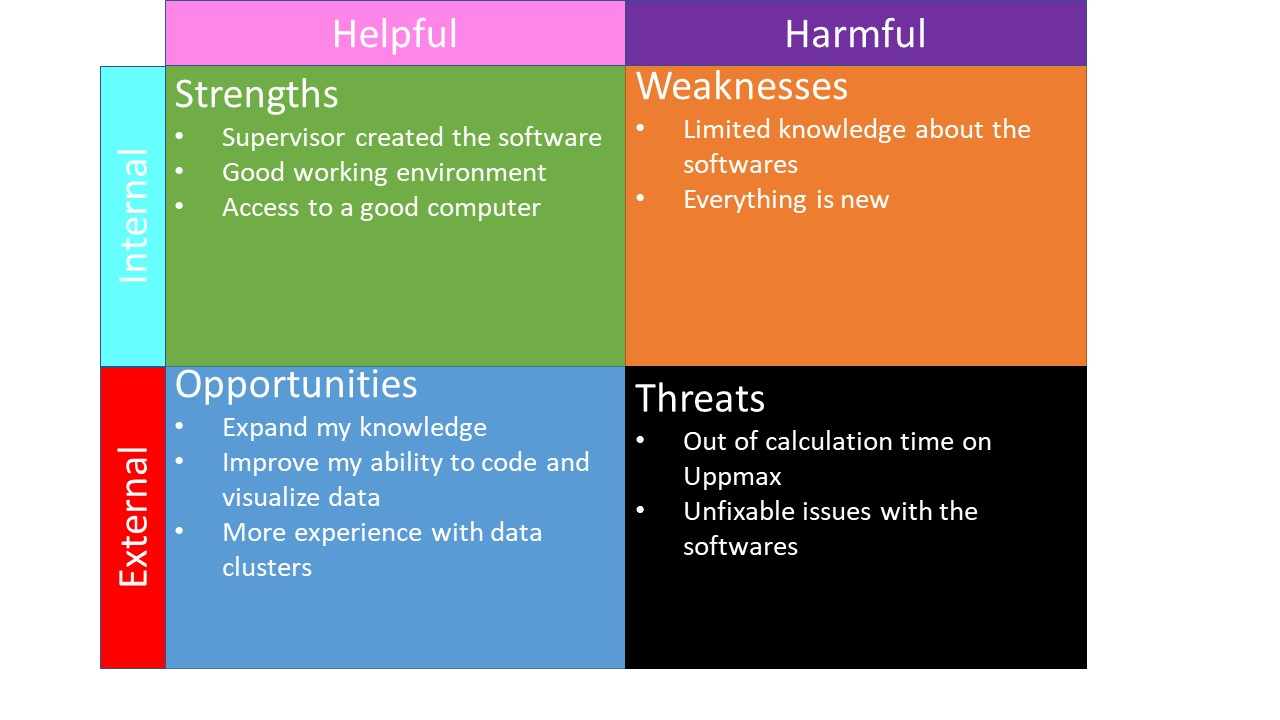
\includegraphics[width=\textwidth,height=\textheight,keepaspectratio]{Pictures/SWOT.jpg}
    \caption{SWOT analysis}
\end{figure}
